
\section{应用}
\label{sec:applications}

\subsection{\trFundamentalGroup{}与\trHomology{}（第二部分）}
\label{subsec:fundamental-group-homology-2}

现在我们将兑现\cref{subsec:fundamental-group-homology-1}中的预告，证明：\trSimplyConnected\trManifold{}的 $H_1$ 为零。

\begin{proposition}\label{thm:simply-connected-hm1-zero}
若 $V$ 是\trSimplyConnected{}的，则 $HM_1(V;\ZZ/2)=0$。
\end{proposition}

\begin{proof}
我们利用 $V$ 上的一个\trMorse--\trSmale{}对 $(f,X)$。先来描述 $V$ 中的那些 1 维\trCycle，也就是说，$C_1(f)$ 中那些满足 $\partial_X\alpha=0$ 的元素 $\alpha$。它们是\trIndex{}为 $1$ 的诸\trCriticalPoint{}的线性组合：
\[
\alpha=a_1+\dots+a_k\text{。}
\]
此外，$\partial_X a_1+\dots+\partial_X a_k=0$。对于一个\trIndex{}为 $1$ 的\trCriticalPoint{} $a$，
\[
\partial_X a=c_1+c_2\text{，}
\]
其中 $c_1$ 与 $c_2$ 是两个\trIndex{}为 $0$ 的\trCriticalPoint，二者未必不同（\cref{fig:index-one-cycles}）：$a$ 的\trUnstableManifold{}是一个维数为 $1$ 的\trOpen\trDisk，而我们可以继续应用\cref{thm:classification-circle-interval}。

\setcounter{figure}{4}%
\begin{figure}[htbp]
\centering
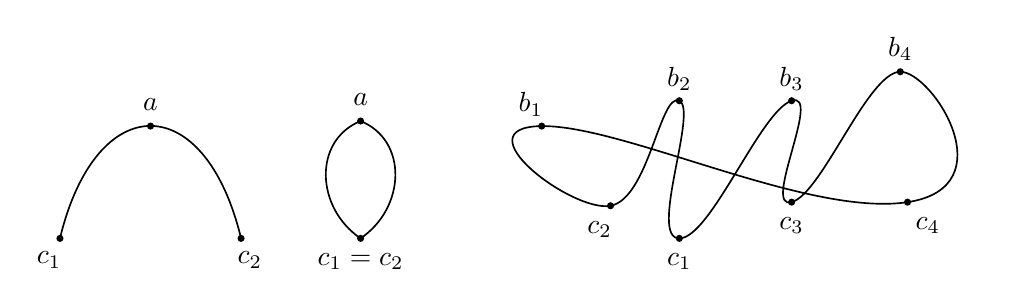
\begin{tikzpicture}[line width=0.6pt,scale=0.92]
  \begin{scope}[shift={(0,0)}]
    \draw (0,0) .. controls (0.5,2.07) and (2.0,2.07) .. (2.5,0);
    \fill (0,0) circle (1.4pt);
    \fill (1.25,1.55) circle (1.4pt);
    \fill (2.5,0) circle (1.4pt);
    \node at (1.25,1.85) {$a$};
    \node at (-0.15,-0.3) {$c_1$};
    \node at (2.62,-0.3) {$c_2$};
  \end{scope}
  \begin{scope}[shift={(4.15,0)}]
    \draw (0,0) .. controls (-0.62,0.42) and (-0.66,1.35) .. (0,1.62)
              .. controls (0.66,1.35) and (0.62,0.42) .. (0,0);
    \fill (0,1.62) circle (1.4pt);
    \fill (0,0) circle (1.4pt);
    \node at (0,1.92) {$a$};
    \node at (0,-0.32) {$c_1=c_2$};
  \end{scope}
  \begin{scope}[shift={(6.3,0)}]
    \draw plot[smooth cycle,tension=1] coordinates{
      (0.35,1.55) (1.3,0.45) (2.25,1.9) (2.25,0.0)
      (3.8,1.9) (3.8,0.5) (5.3,2.3) (5.4,0.5)};
    \fill (0.35,1.55) circle (1.4pt);
    \fill (1.3,0.45) circle (1.4pt);
    \fill (2.25,1.9) circle (1.4pt);
    \fill (2.25,0.0) circle (1.4pt);
    \fill (3.8,1.9) circle (1.4pt);
    \fill (3.8,0.5) circle (1.4pt);
    \fill (5.3,2.3) circle (1.4pt);
    \fill (5.4,0.5) circle (1.4pt);
    \node at (0.2,1.85) {$b_1$};
    \node at (1.15,0.12) {$c_2$};
    \node at (2.25,2.2) {$b_2$};
    \node at (2.25,-0.32) {$c_1$};
    \node at (3.8,2.2) {$b_3$};
    \node at (3.8,0.18) {$c_3$};
    \node at (5.3,2.62) {$b_4$};
    \node at (5.68,0.18) {$c_4$};
  \end{scope}
\end{tikzpicture}
\caption{}
\label{fig:index-one-cycles}
\end{figure}

于是，我们的\trCycle{} $\alpha$ 就是若干\trCycle
\[
\beta=b_1+\dots+b_s
\]
之和，其中 $\partial b_i=c_i+c_{i+1}$，而 $c_1,\dotsc,c_s$ 为诸局部极小点（约定 $c_{s+1}=c_1$），如\cref{fig:index-one-cycles}所示。

这样的一个 $\beta$ 给出\trCircle{} $S^1$ 到 $V$ 中的一个\trEmbedding{} $u_\beta$，使得函数 $g_\beta=f\circ u_\beta$ 以诸 $c_i$ 为局部极小点、以诸 $b_i$ 为局部极大点。\footnote{译注：闭圈（$c_1=c_2$ 情形）的两段弧在极小点拼接处一般有折角（两条射线未必共线），故 $u_\beta$ 一般只是分段\trSmooth{}的连续\trInjective，未必是 $\cC^\infty$ \trEmbedding；严格处理须先在诸局部极小点的邻域内作\trSmooth{}替换并验证\trHomology{}类不变，或先把\trFunctoriality{}拓展到连续映射；原书径称之为\trEmbedding，照排于此。——译者注}$\operatorname{Ker}\partial\subset C_1(f)$ 的一个基中的每个 $\beta$ 都定义了一个（\trInjective{}的）\trComplex\trMorphism
\[
(u_\beta)_\bullet\colon C_\bullet(g_\beta,X_\beta)\longrightarrow C_\bullet(f,X)
\]
（$X_\beta$ 是 $S^1$ 上的一个\trVectorField，其像是 $X$ 的限制），使得
\[
(u_\beta)_\star\colon HM_1(S^1;\ZZ/2)\longrightarrow HM_1(V;\ZZ/2)
\]
的\trImage{}是由 $\beta$ 的类所生成的那个子空间。

在 $V$ \trSimplyConnected{}的条件之下，每个映射 $v\colon S^1\to V$ 都能扩张成一个映射 $\widetilde v\colon D^2\to V$。特别地，在\trHomology{}中，
\[
u_\beta\colon S^1\hookrightarrow D^2\xrightarrow{\ \widetilde u_\beta\ }V
\]
给出一个分解
\[
(u_\beta)_\star\colon HM_1(S^1;\ZZ/2)\longrightarrow HM_1(D^2;\ZZ/2)
  \xrightarrow{\ (\widetilde u_\beta)_\star\ }HM_1(V;\ZZ/2)\text{，}
\]
于是 $\beta$ 的类来自 $HM_1(D^2;\ZZ/2)=0$，从而为零。
\end{proof}

\subsection{\trBrouwer{}\trFixedPoint{}定理}
\label{subsec:brouwer-via-homology}

下面给出\trBrouwer{}定理（\cref{thm:brouwer-fixed-point}）的另一个证明。

\begin{proof}[\cref{thm:brouwer-fixed-point}的证明]
与先前的证明一样，我们一开始先化归到 $\varphi$ 为 $\cC^\infty$ 映射的情形，并假定它没有\trFixedPoint。于是我们构造一个收缩
\[
r\colon D^n\longrightarrow S^{n-1}
\]
它把 $x\in D^n$ 送到\trSphere{} $S^{n-1}$ 与那条从 $\varphi(x)$ 出发且穿过 $x$ 的射线的交点。这样一来，如果 $x$ 是\trSphere{}上的一个点，它就原地不动。映射 $r$ 满足
\[
r\circ j=\mathrm{Id}\colon S^{n-1}\hookrightarrow D^n\longrightarrow S^{n-1}\text{。}
\]
因此，复合 $r_\star\circ j_\star$，
\[
HM_{n-1}(S^{n-1};\ZZ/2)\longrightarrow HM_{n-1}(D^n;\ZZ/2)
  \longrightarrow HM_{n-1}(S^{n-1};\ZZ/2)\text{，}
\]
也必须是从 $\ZZ/2$ 到 $\ZZ/2$ 的恒等映射；然而，正如我们在\cref{thm:disk-relative-homology}中所指出的，$HM_{n-1}(D^n;\ZZ/2)=0$。这个矛盾蕴含了\trFixedPoint{}的存在性。
\end{proof}

用同样的方式，我们可以证明：若 $k<n$，则不存在从\trSphere{} $S^n$ 到它的一个子\trSphere{} $S^k\subset S^n$ 上的收缩。否则，在\trMorseHomology{}中，复合
\[
S^k\xrightarrow{\ \ i\ \ }S^n\xrightarrow{\ \ r\ \ }S^k\text{，}
\]
就会给出
\[
\begin{array}{ccccc}
HM_k(S^k;\ZZ/2) & \xrightarrow{\ \ i_\star\ \ } & HM_k(S^n;\ZZ/2)
  & \xrightarrow{\ \ r_\star\ \ } & HM_k(S^k;\ZZ/2)\\[3pt]
\ZZ/2 & \longrightarrow & 0 & \longrightarrow & \ZZ/2\text{，}
\end{array}
\]
这是一个本应当为恒等映射的零映射。

\subsection{\trProjectiveSpace{}的模 2 \trHomology}
\label{subsec:mod2-homology-projective-space}

让我们考虑\trSphere{}
\[
S^n=\{x\in\RR^{n+1}\mid \|x\|^2=1\}
\]
及其在等价关系 $x\sim-x$ 之下作商的结果，也就是 $\CP^n(\RR)$，即维数为 $n$ 的实\trProjectiveSpace。自然投影 $S^n\to\CP^n(\RR)$ 记作 $p$。

设 $f$ 是 $\CP^n(\RR)$ 上的一个\trMorseFunction。函数 $f\circ p$ 是 $S^n$ 上的一个\trMorseFunction（在局部，$S^n$ 与 $\CP^n(\RR)$ 没有什么两样）。在 $f$ 的每个\trCriticalPoint{} $p(a)$ 的上方，它都有两个\trIndex{}为 $k$ 的\trCriticalPoint：$a$ 与 $-a$。

同样地，若 $X$ 是\trAdapted{}于 $f$ 的一个\trPseudogradient{}场，则存在 $S^n$ 上的一个\trVectorField{} $\widetilde X$，它是 $f\circ p$ 的\trPseudogradient{}场，并且使得对 $S^n$ 上的每个 $x$，
\[
T_x(p)(\widetilde X_x)=X_{p(x)}\text{。}
\]
于是，$\widetilde X$ 的诸\trTrajectory{}都投影成 $X$ 的诸\trTrajectory。再者，如果我们假定 $X$ 满足\trSmaleCondition，那么 $\widetilde X$ 也同样满足。特别地，对 $f\circ p$ 的所有\trIndex{}相邻的\trCriticalPoint{} $a$ 与 $b$，我们有
\[
n_{\widetilde X}(a,b)=n_{\widetilde X}(-a,-b)\text{。}
\]

\begin{figure}[htbp]
\centering
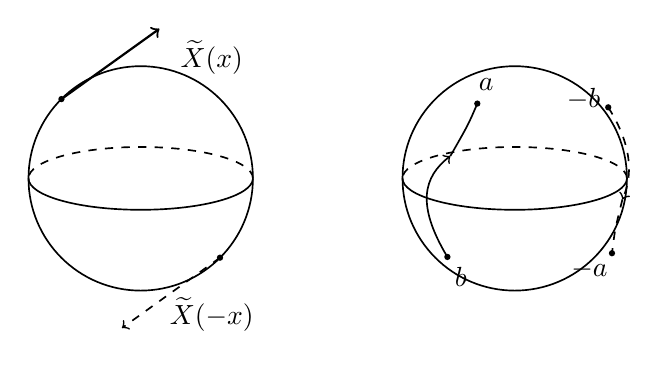
\begin{tikzpicture}[line width=0.6pt,scale=0.95]
  \begin{scope}[shift={(0,0)}]
    \draw (0,0) circle (1.5);
    \draw[dashed] (1.5,0) arc[start angle=0,end angle=180,x radius=1.5,y radius=0.42];
    \draw (-1.5,0) arc[start angle=180,end angle=360,x radius=1.5,y radius=0.42];
    \draw[->,line width=0.8pt] (-1.06,1.06) -- (0.25,2.0);
    \fill (-1.06,1.06) circle (1.2pt);
    \node at (0.95,1.62) {$\widetilde X(x)$};
    \draw[dashed,->] (1.06,-1.06) -- (-0.25,-2.0);
    \fill (1.06,-1.06) circle (1.2pt);
    \node at (0.95,-1.82) {$\widetilde X(-x)$};
  \end{scope}
  \begin{scope}[shift={(5.0,0)}]
    \draw (0,0) circle (1.5);
    \draw[dashed] (1.5,0) arc[start angle=0,end angle=180,x radius=1.5,y radius=0.42];
    \draw (-1.5,0) arc[start angle=180,end angle=360,x radius=1.5,y radius=0.42];
    \draw[->] (-0.9,-1.05) .. controls (-1.32,-0.35) and (-1.22,0.02) .. (-0.86,0.3);
    \draw (-0.86,0.3) .. controls (-0.62,0.72) .. (-0.5,1.0);
    \fill (-0.9,-1.05) circle (1.2pt);
    \fill (-0.5,1.0) circle (1.2pt);
    \draw[dashed,->] (1.25,0.95) .. controls (1.6,0.4) and (1.56,0.0) .. (1.44,-0.28);
    \draw[dashed] (1.44,-0.28) .. controls (1.34,-0.68) .. (1.3,-1.0);
    \fill (1.25,0.95) circle (1.2pt);
    \fill (1.3,-1.0) circle (1.2pt);
    \node at (-0.38,1.25) {$a$};
    \node at (-0.72,-1.32) {$b$};
    \node at (0.92,1.06) {$-b$};
    \node at (1.0,-1.22) {$-a$};
  \end{scope}
\end{tikzpicture}
\caption{}
\label{fig:sphere-covering-lift}
\end{figure}

公式 $\alpha\mapsto p(\alpha)$ 定义了一个\trComplex\trMorphism{} $(C_k(\widetilde f),\partial_{\widetilde X})\to(C_k(f),\partial_X)$，我们把它记作 $p_\star$（这其实算不上滥用记号：正如可以用诸\trEmbedding{}来验证的，它确实是那个由可微映射 $p$ 所定义的 $p_\star$）。同样地，公式
\[
p(a)\longmapsto a+(-a)
\]
定义了一个线性映射
\[
p^!\colon C_k(f)\longrightarrow C_k(\widetilde f)\text{。}
\]
若 $\alpha=p(a)=p(-a)$ 是 $f$ 的一个\trCriticalPoint，那么我们有
\[
\begin{aligned}
\partial_{\widetilde X}(p^!\alpha)
  &=\partial_{\widetilde X}(a)+\partial_{\widetilde X}(-a)\\
  &=\sum_b n_{\widetilde X}(a,b)\,b+\sum_c n_{\widetilde X}(-a,c)\,c\\
  &=\sum_b n_{\widetilde X}(a,b)\,b+\sum_b n_{\widetilde X}(-a,-b)\,(-b)\text{。}
\end{aligned}
\]
但是，从 $a$ 到 $b$ 存在一条\trTrajectory，当且仅当从 $-a$ 到 $-b$ 存在一条\trTrajectory，于是这个和等于
\[
\begin{aligned}
\partial_{\widetilde X}(p^!\alpha)
  &=\sum_b n_{\widetilde X}(a,b)\,b+\sum_{-b} n_{\widetilde X}(-a,-b)\,(-b)\\
  &=\sum_b n_{\widetilde X}(a,b)\,\bigl(b+(-b)\bigr)\\
  &=\sum_\beta n_X(\alpha,\beta)\,\bigl(b+(-b)\bigr)\\
  &=\sum_\beta n_X(\alpha,\beta)\cdot p^!(\beta)=p^!(\partial_X\alpha)\text{。}
\end{aligned}
\]
（其中 $p(b)=\beta$。）因此，$p^!$ 是一个\trComplex\trMorphism
\[
p^!\colon(C_k(f),\partial_X)\longrightarrow(C_k(f\circ p),\partial_{\widetilde X})\text{。}
\]
复合
\[
(C_k,\partial_X)\xrightarrow{\ \ p^!\ \ }(C_k(f\circ p),\partial_{\widetilde X})
  \xrightarrow{\ \ p_\star\ \ }(C_k(f),\partial_X)
\]
先把\trCriticalPoint{} $\alpha$ 送到 $a+(-a)$，随后又把它送到
\[
p(a)+p(-a)=2\alpha=0\text{。}
\]
更确切地说，我们有\trComplex{}的一个\trExact{}列
\[
0\longrightarrow(C_k(f),\partial_X)\xrightarrow{\ \ p^!\ \ }(C_k(f\circ p),\partial_{\widetilde X})
  \xrightarrow{\ \ p_\star\ \ }(C_k(f),\partial_X)\longrightarrow 0\text{。}
\]
实际上，$\widetilde f$ 的诸\trCriticalPoint{}的一个线性组合 $a_1+\dots+a_k$ 被送到 $p(a_1)+\dots+p(a_k)$，它只有在这个和中 $f$ 的每个\trCriticalPoint{}都出现两次时才可能为零，也就是说，只有当
\[
a_1+\dots+a_k=a_{i_1}+(-a_{i_1})+\dots+a_{i_r}+(-a_{i_r})
\]
时才可能为零，换言之，只有当这个元素属于 $p^!$ 的\trImage{}时才可能为零。

于是，我们得到了\trComplex{}的一个\trExact{}列，它不出所料地给出下面的\trMorseHomology{}\trLongExactSequence
\[
\begin{tikzcd}[column sep=1.35cm,row sep=1.15cm]
HM_k(\CP^n(\RR);\ZZ/2) \ar[r] & HM_k(S^n;\ZZ/2) \ar[r]
  & HM_k(\CP^n(\RR);\ZZ/2) \ar[from=1-3,to=2-1,shift right=1.5mm,"\partial"] \\
HM_{k-1}(\CP^n(\RR);\ZZ/2) \ar[r] & \cdots
\end{tikzcd}
\]

由此推出，\trConnectingHomomorphism
\[
\partial\colon HM_k(\CP^n(\RR);\ZZ/2)\longrightarrow HM_{k-1}(\CP^n(\RR);\ZZ/2)
\]
在 $0\le k\le n$ 时是一个\trIsomorphism。于是我们就证明了下面的结果。

\begin{theorem}\label{thm:mod2-hm-projective-space}
我们有 $HM_k(\CP^n(\RR);\ZZ/2)\cong\ZZ/2$，其中 $0\le k\le n$。\noqed
\end{theorem}

至于整系数的\trHomology（其中的诸\trOrientation{}问题必须谨慎对待）；参见\cref{ex:ch04-24}与\cref{ex:ch04-25}。

下面给出这个\trExact{}列的\trConnectingHomomorphism{}的一个显式描述。要把它确定下来，只需循着它的抽象定义走一遍。我们先来选定 $S^n$ 的一个半球——这次不妨换个口味，就选南半球。设 $\alpha$ 是 $(C_k(f),\partial_X)$ 中的一个\trCycle，
\[
\alpha=\alpha_1+\dots+\alpha_r\text{，}
\]
那么我们在南半球中选取诸 $\alpha_i$ 的\textbf{\trLift}（lift） $a_i$，得到一个和
\[
a=a_1+\dots+a_r
\]
它在 $p_\star$ 下的像正是我们的\trCycle{} $\alpha$。于是，$\partial_{\widetilde X}a$ 是 $\widetilde f$ 的\trIndex{}为 $k-1$ 的诸\trCriticalPoint{}的一个线性组合，形如
\[
\partial_{\widetilde X}a=\sum_{i=1}^{p}\bigl(b_i+(-b_i)\bigr)
\]
其中诸 $b_i$ 都位于南半球中。此时我们便有\footnote{译注：原书左端印作 $\partial[a]$；但 $a=a_1+\dots+a_r$ 只是诸 $\alpha_i$ 在南半球中的\trLift{}之和，一般并非\trCycle（$\partial_{\widetilde X}a=\sum_{i=1}^{p}\bigl(b_i+(-b_i)\bigr)\neq 0$），故 $[a]$ 未必有定义；左端应作 $\partial[\alpha]$（$\alpha$ 才是 $(C_k(f),\partial_X)$ 中的\trCycle）；此处径改。——译者注}
\[
\partial[\alpha]=\bigl[p(b_1)+\dots+p(b_p)\bigr]\text{。}
\]

\subsection{\trBorsuk{}--\trUlam{}定理}
\label{subsec:borsuk-ulam-theorem}

现在让我们来证明下面这个著名的定理。

\begin{theorem}[\trBorsuk{}--\trUlam]\label{thm:borsuk-ulam}
不存在任何连续映射
\[
\varphi\colon S^n\longrightarrow S^{n-1}
\]
使得对每个 $x$ 都有 $\varphi(-x)=-\varphi(x)$。
\end{theorem}

这个定理有着若干或多或少颇为有趣、却并不怎么严肃的应用（例如，一个令人着迷的事实：任一时刻，地球上总存在两个\textbf{\trAntipodal{}点}（antipodal points），具有相同的温度与大气压）。\footnote{译注：即下文\cref{thm:temperature-pressure}的气象学版本，作者随后戏称之为“温度--气压”定理。}

\begin{corollary}\label{thm:odd-map-vanishes}
设 $\psi\colon S^n\to\RR^n$ 是一个连续映射，使得对每个 $x$ 都有 $\psi(-x)=-\psi(x)$。那么 $\psi$ 在 $S^n$ 上至少有一个零点。
\end{corollary}

\begin{proof}
这是因为，倘若 $\psi$ 处处都不为零，那么它就会定义一个取值于 $S^{n-1}$ 中的映射 $\varphi=\psi/\|\psi\|$，而这正是该定理所禁止的。
\end{proof}

下面是“温度--气压”定理。

\begin{corollary}\label{thm:temperature-pressure}
对每个映射 $\psi\colon S^n\to\RR^n$，至少存在 $S^n$ 的一个点 $x$，使得 $\psi(x)=\psi(-x)$。
\end{corollary}

\begin{proof}
特别要注意的是，并不存在任何从 $S^n$ 到 $\RR^n$ 中的\trInjective。这个推论可以借助考虑 $\varphi(x)=\psi(x)-\psi(-x)$ 来证明。
\end{proof}

\begin{corollary}\label{thm:cover-by-closed-antipodal}
设 $F_1,F_2,\dotsc,F_{n+1}$ 是\trSphere{} $S^n$ 的非空\trClosed{}子集，其并为整个\trSphere。那么诸 $F_i$ 之一必含有两个\trAntipodal{}点。
\end{corollary}

\begin{proof}
只需利用映射
\[
\psi(x)=\bigl(d(x,F_1),d(x,F_2),\dotsc,d(x,F_n)\bigr)\text{。}\qedhere
\]
\end{proof}

\begin{proof}[\cref{thm:borsuk-ulam}的证明]
当然了，正如\trBrouwer{}定理的情形一样，我们将要证明的是：不存在任何具有所需性质的 $\cC^\infty$ 映射（连续映射的结果由它可得）。一个具有所述性质的映射 $\varphi$ 将会诱导出一个映射 $\psi\colon\CP^n(\RR)\to\CP^{n-1}(\RR)$，我们将证明后者不可能存在。

那么，设 $\psi$ 是从 $\CP^n(\RR)$ 到 $\CP^{n-1}(\RR)$ 的一个 $\cC^\infty$ 映射。考虑图
\[
\begin{tikzcd}[column sep=1.2cm,row sep=1.35cm]
HM_k(\CP^n(\RR);\ZZ/2) \ar[r,"\psi_\star"] \ar[d,"\partial"']
  & HM_k(\CP^{n-1}(\RR);\ZZ/2) \ar[d,"\partial"] \\
HM_{k-1}(\CP^n(\RR);\ZZ/2) \ar[r,"\psi_\star"']
  & HM_{k-1}(\CP^{n-1}(\RR);\ZZ/2)
\end{tikzcd}
\]
其中\trConnectingHomomorphism{} $\partial$ 已在\cref{subsec:mod2-homology-projective-space}小节中定义。我们将从这幅图推出：
\[
\psi_\star\colon HM_n(\CP^n(\RR);\ZZ/2)\longrightarrow HM_n(\CP^{n-1}(\RR);\ZZ/2)
\]
非零——而这是荒谬的，因为后一个群是零。我们用归纳法证明：
\[
\psi_\star\colon HM_k(\CP^n(\RR);\ZZ/2)\longrightarrow HM_k(\CP^{n-1}(\RR);\ZZ/2)
\]
在 $k\le n-1$ 时是一个\trIsomorphism。

当 $k=0$ 时，这是一个十分一般的事实，它来自下一条引理。

\begin{lemma}\label{thm:hm0-identity-map}
设 $V$ 与 $W$ 是\trConnected\trManifold，并设 $u\colon V\to W$ 是一个 $\cC^\infty$ 映射。那么，由它诱导的映射
\[
u_\star\colon HM_0(V;\ZZ/2)\longrightarrow HM_0(W;\ZZ/2)
\]
是恒等映射。
\end{lemma}

\begin{proof}
我们使用\cref{thm:inclusion-induced-isomorphism} 的记号。按定义，
\[
u_\star=(i_0^{-1})_\star\circ(u,\psi)_\star\text{，}
\]
其中 $\psi$ 是一个\trEmbedding{} $V\to D^N$。\footnote{译注：原书此处印作 “where $\psi$ in an embedding”；疑应为 “where $\psi$ is an embedding”（in→is，显见排印笔误）；此处径改。——译者注}根据\cref{thm:inclusion-induced-isomorphism}，$i_0\colon W\to D^N\times W$ 在\trHomology{}中诱导一个\trIsomorphism。于是，只需在 $u$ 是\trEmbedding{}的情形下证明本引理。

我们在\cref{thm:hm0-connected-manifold}中已经证明：$HM_0(V;\ZZ/2)$ \trIsomorphic{}于 $\ZZ/2$，并且由 $V$ 上一个\trMorseFunction{}的任意一个\trIndex{}为 $0$ 的\trCriticalPoint{} $c$ 所生成。另一方面，若 $u\colon V\to W$ 是一个\trEmbedding，则\cref{thm:morse-smale-extension} 的证明表明 $u_\star(c)=u(c)$，其中 $u(c)$ 是 $f\circ u^{-1}$ 到 $W$ 上的一个适当延拓的\trIndex{}为 $0$ 的\trCriticalPoint。引理得证。
\end{proof}

现在假设：对某个 $k\le n-1$，$\psi_\star$ 在 $HM_{k-1}$ 的层级上诱导一个\trIsomorphism。假定上图交换。由于两个竖直箭头都是\trIsomorphism，根据\cref{thm:mod2-hm-projective-space}，$\psi_\star$ 在 $HM_k$ 的层级上也诱导一个\trIsomorphism。

现在考虑 $k=n$ 情形下的这幅图。左边的竖直箭头 $\partial$ 是一个\trIsomorphism（仍由\cref{thm:mod2-hm-projective-space}），于是 $\psi_\star\circ\partial$ 是\trIsomorphism。因此
\[
\psi_\star\colon HM_n(\CP^n(\RR);\ZZ/2)\longrightarrow HM_n(\CP^{n-1}(\RR);\ZZ/2)
\]
非零，而这是荒谬的。

余下还需证明这幅图是交换的。设 $\Gamma\colon\CP^n(\RR)\to D^N$ 是一个\trEmbedding。按定义，$\psi_\star=(i_0^{-1})_\star(\Gamma,\psi)_\star$，于是只需证明图
\[
\begin{tikzcd}[column sep=1.15cm,row sep=1.35cm]
HM_k(\CP^n(\RR);\ZZ/2) \ar[r,"{(\Gamma,\psi)_\star}"] \ar[d,"\partial"']
  & HM_k(D^N\times\CP^{n-1}(\RR);\ZZ/2) \ar[d,"\partial"] \\
HM_{k-1}(\CP^n(\RR);\ZZ/2) \ar[r,"{(\Gamma,\psi)_\star}"']
  & HM_{k-1}(D^N\times\CP^{n-1}(\RR);\ZZ/2)
\end{tikzcd}
\]
与图
\[
\begin{tikzcd}[column sep=1.15cm,row sep=1.35cm]
HM_k(\CP^{n-1}(\RR);\ZZ/2) \ar[r,"{(i_0)_\star}"] \ar[d,"\partial"']
  & HM_k(D^N\times\CP^{n-1}(\RR);\ZZ/2) \ar[d,"\partial"] \\
HM_{k-1}(\CP^{n-1}(\RR);\ZZ/2) \ar[r,"{(i_0)_\star}"']
  & HM_{k-1}(D^N\times\CP^{n-1}(\RR);\ZZ/2)
\end{tikzcd}
\]
是交换的，其中
\[
\partial\colon HM_k(D^N\times\CP^{n-1}(\RR);\ZZ/2)
  \longrightarrow HM_{k-1}(D^N\times\CP^{n-1}(\RR);\ZZ/2)
\]
由一个类似的\trComplex\trExact{}列所定义。

第二幅图显然是交换的：若我们使用 $D^N$ 上的\trMorseFunction{} $x\mapsto\|x\|^2$，则两个\trComplex{}的\trExact{}列完全相同，并且 $(i_0)_\star=\mathrm{Id}$。现在我们来考虑第一幅图。

回忆一下，$\psi$ 是由一个映射
\[
\varphi\colon S^n\longrightarrow S^{n-1}
  \qquad\text{满足}\qquad \varphi(-x)=-\varphi(x)
\]
所定义的。这就蕴含着：
\[
(\Gamma\circ p,\varphi)\colon S^n\longrightarrow D^N\times S^{n-1}
\]
是一个\trEmbedding。现在，我们在 $\CP^n(\RR)$ 上取一个\trMorse--\trSmale{}对 $(f,X)$。像先前那样，把它\trLift{}为 $S^n$ 上的一个\trMorse--\trSmale{}对 $(f\circ p,\widetilde X)$。然后，正如\cref{thm:morse-smale-extension} 的证明中那样，我们把 $\bigl(f\circ(\Gamma,\psi)^{-1},T(\Gamma,\psi)X\bigr)$ 延拓为 $(\overline f,\overline X)$，即 $D^N\times\CP^{n-1}(\RR)$ 上的一个\trMorse--\trSmale{}对。我们再把 $(\overline f,\overline X)$ \trLift{}为 $D^N\times S^{n-1}$ 上的 $(\overline f\circ p,\widetilde{\overline X})$（它是 $\bigl(f\circ p\circ(\Gamma\circ p,\varphi)^{-1},T(\Gamma\circ p,\varphi)\widetilde X\bigr)$ 的一个延拓）。\footnote{译注：原书此处印作 $T(\Gamma,\varphi)\widetilde X$；$\Gamma$ 定义于 $\CP^n(\RR)$ 之上，而 $\widetilde X$ 是 $S^n$ 上的\trVectorField，按前句的\trEmbedding{} $(\Gamma\circ p,\varphi)\colon S^n\to D^N\times S^{n-1}$ 应作 $T(\Gamma\circ p,\varphi)\widetilde X$；此处径改。——译者注}这就给出了图
\[
\begin{tikzcd}[column sep=0.92cm,row sep=1.55cm]
0 \ar[r] & C_\bullet(f,X) \ar[r,"p^!"] \ar[d,"{(\Gamma,\psi)_\bullet}"']
  & C_\bullet(f\circ p,\widetilde X) \ar[r,"p"] \ar[d,"{(\Gamma\circ p,\varphi)_\bullet}"]
  & C_\bullet(f,X) \ar[r] \ar[d,"{(\Gamma,\psi)_\bullet}"] & 0 \\
0 \ar[r] & C_\bullet(\overline f,\overline X) \ar[r,"p^!"']
  & C_\bullet(\overline f\circ p,\widetilde{\overline X}) \ar[r,"\overline p"']
  & C_\bullet(\overline f,\overline X) \ar[r] & 0
\end{tikzcd}
\]
其中诸水平\trExact{}列、诸交换方形与诸竖直箭头均由\cref{thm:morse-smale-extension} 所定义。利用\trConnectingHomomorphism{} $\partial$ 的定义，随即容易验证这幅图是交换的。请注意，当我们把两幅图中左侧的竖直箭头等同起来时，我们实际上隐含地使用了这样一个事实：$\partial$ 不依赖于 $D^N\times\CP^{n-1}(\RR)$ 上\trMorse--\trSmale{}对的选取。这是因为 $\partial$ 是一个\trIsomorphism，而 $\ZZ/2$ 到其自身的\trIsomorphism{}只有恒等映射。
\end{proof}
